\documentclass{fast-nuces-bs}

\usepackage{blindtext}
\usepackage{mathptmx}% Times Roman font
\usepackage[T1]{fontenc}
\usepackage{lipsum} 
\usepackage{sectsty}
\usepackage{tikz-uml}
\usepackage{titlesec}
\usepackage{tikz}
\usetikzlibrary{shapes, arrows, positioning, calc}

\tikzstyle{block} = [rectangle, draw, fill=blue!15, text centered, rounded corners, minimum height=2em, minimum width=6cm]
\tikzstyle{line} = [draw, thick, -latex']
\tikzstyle{side} = [rectangle, draw, fill=green!15, text centered, rounded corners, minimum height=2em, minimum width=3cm]

% Information about the Thesis 
% -----------------------------------------------------------------------------
% (All are compulsory, do not delete any line other than author Information)
% For e.g., usually there are 3 students in a group, so leave authorone, 
% authortwo, and authorthree, and delete authorfour.
%%%%%%%%%%%%%%%%%%%%%%%%%%%%%%%%%%%%%%%%%%%%%%%%%%%%%%%%%%%%%%%%%%%%%%%%%%%%%%%
\department{Department of Computer Science}
\faculty{Computer Science}
\degreeyear{2026}
\degreemonth{June}
\degreename{Computer Science}
\campuscity{Islamabad}
\authorone{Arrij Fawwad}{22I-0755}
\authortwo{Hamna Arshad}{22I-1098}
\authorthree{Zubair Khalid}{22I-2475}
\supervisor{Dr. Arshad Islam}
\sessionduration{2022-2026}
\cosupervisor{Mr. Usama Imtiaz}
\deanname{Dr. Jawwad Ahmed Shamsi}
\directorname{Dr. Waseem Shahzad}
\hodname{Dr. Arshad Islam}
%\fypcoordinatorname{Name of FYP Coordinator}
\title{A Multi-Agent Requirement Engineering System - MARS}
%%%%%%%%%%%%%%%%%%%%%%%%%%%%%%%%%%%%%%%%%%%%%%%%%%%%%%%%%%%%%%%%%%%%%%%%%%%%%%%

%%%%%%%%%%%%%%%%%%%%%%%%%%%%%%%%%%%%%%%%%%%%%%%%%%%%%%%%%%%%%%%%%%%%%%%%%%%%%%
% Former document starts below this
\begin{document}


\chapter{Introduction}
\label{sec:introduction}
\section{Problem Statement}
\vspace{-0.5cm} 
Software development projects often face challenges not due to technical shortcomings, but because of poorly defined requirements that compromise the foundation of the system. Requirements engineering (RE) is widely recognized as one of the most critical yet error-prone phases of the development lifecycle. Conventional approaches rely heavily on manual effort and the availability of experts, making the process time-consuming, inconsistent, and prone to human error. This creates barriers for non-specialists, reduces efficiency, and increases the likelihood of costly mistakes.
The Standish Group’s CHAOS Report highlights this risk, showing that a clear statement of requirements contributes 13\% to project success, while 12.3\% of challenged projects are caused by incomplete or unclear specifications \cite{1}. These figures underline how even small lapses in requirement clarity can trigger significant delays, rework, and in many cases, outright project failure. Traditional RE practices often produce Software Requirements Specification (SRS) documents that suffer from ambiguity, inconsistency, and conflicts, leading to miscommunication among stakeholders.
Research by IBM underscores the importance of accuracy at the outset, showing that fixing a defect in production can cost up to 100 times more than correcting it during the requirements phase \cite{2}.
Ultimately, the recurring problems of incompleteness, ambiguity, and inconsistency in requirements undermine software quality and project success. These challenges highlight the urgent need for an intelligent, systematic solution that enhances requirement clarity, reduces errors, and streamlines the transition to development.

\section{Motivation}
The motivation for this project arises from the critical role that requirements engineering plays in determining software success and the persistent challenges associated with it. Studies indicate that around 56\% of software defects originate in the requirements phase \cite{3}, showing how errors at this stage create the most damaging ripple effects throughout development. These figures highlight the urgency of improving practices that ensure clarity, completeness, and consistency in requirements.
At the same time, the requirements management market is projected to reach USD 3.2 billion by 2033 \cite{4}, with AI integration emerging as a key driver of growth. This trend reflects a broader industry recognition that traditional approaches are insufficient and that intelligent, automated support is increasingly essential. The combination of high technical risk and growing market demand provides strong motivation to explore solutions that enhance requirements engineering practices.
Ultimately, the driving motivation behind this project is the opportunity to reduce costly downstream errors, improve project outcomes, and contribute to the evolving landscape of requirements engineering by addressing one of the most persistent pain points in software development.

\section{Problem Solution}
The proposed software, MARS (Multi-Agent Requirements Engineering System), is an AI-driven assistant designed to directly address the recurring challenges identified in the requirements engineering process. Traditional practices often result in incomplete, ambiguous, or conflicting specifications, which increase rework, miscommunication, and project failures. To overcome these limitations, MARS integrates automation, reasoning, and conversational interaction into a unified platform, ensuring requirements are captured, validated, and organized with greater accuracy and efficiency.
The first objective of MARS is to engage users in a conversational elicitation process, enabling both technical and non-technical stakeholders to express requirements without the need for specialized expertise. Second, the system performs automated quality assurance, detecting ambiguity, conflicts, duplicates, and non-atomic requirements at the earliest stage, thereby reducing costly downstream errors. Third, it ensures proper categorization of requirements into functional and non-functional types, aligning them with established software engineering practices.
Beyond validation and classification, MARS contributes to agile development workflows by generating user stories from refined requirements, making them directly actionable for development teams. Another key goal is to produce editable, standards-compliant Software Requirements Specification (SRS) documents, which include core sections such as Introduction, Scope, Functional and Non-Functional Requirements, and Glossary. At the same time, MARS allows the inclusion of elements, added and customized directly by users through the integrated chatbot, ensuring the document remains adaptable to project-specific needs.
By meeting these objectives, MARS minimizes the reliance on manual effort, reduces the expertise barrier for high-quality requirements engineering, and accelerates the process of moving from stakeholder intentions to structured specifications. The ultimate goal is to embed quality at the requirements stage, where errors are most costly, while making professional-grade requirements engineering more accessible, consistent, and adaptable across diverse project environments.

\section{Stake Holders}
\begin{enumerate}
\item Clients / End-Users – Provide the requirements and validate that the final SRS reflects their needs.
\item Business Analysts / Requirements Engineers – Use the system to elicit, refine, and structure requirements into a high-quality specification.
\item Project Managers – Depend on accurate, conflict-free requirements to plan resources, timelines, and deliverables.
\item Software Developers – Rely on the generated user stories and categorized requirements to guide implementation.
\item Quality Assurance (QA) Teams – Use the clarified requirements to design effective test cases and ensure product correctness.
\end{enumerate}

\chapter{Project Description}
\label{ch:description}
\section{Scope}
\vspace{-1.06cm}
The scope of this project is to design and implement an AI-assisted system that supports requirement elicitation, quality assessment, refinement, and partial automation of the Software Requirement Specification (SRS) document. The system will accept user input in text form or document upload, limited to English, and provide a chatbot-based interface to enable natural and guided elicitation of requirements. It will generate context-aware clarifying questions to resolve ambiguities and missing details through iterative interaction with users. Drafted requirements will be automatically analyzed for duplication, conflicts, and classification, with the system suggesting corrections where possible and escalating complex issues to users through human-in-the-loop support. The system will further automate the creation of a partially complete SRS, covering introduction, audience, scope, product perspective, functional and non-functional requirements, glossary, and user classes. Users will be able to select templates, refine sections, and add new requirements with chatbot assistance. Additionally, finalized requirements will be transformed into structured user stories to support agile development processes. However, the scope excludes functionalities such as software coding, testing, graphical modeling, or generating diagrams. It will not support multiple projects simultaneously or collaborative editing, and users will retain full responsibility for final review and validation. The system also does not address hardware or architectural constraints that may impact performance. By focusing specifically on elicitation, refinement, and structured documentation, the project establishes clear boundaries and ensures that users receive AI-driven support for requirement engineering without extending into development or operational activities.

\section{Modules}
The proposed system is divided into the following key modules, each addressing a specific phase of the requirement engineering process and collectively contributing to the automated generation of high-quality software requirement specifications.

\subsection{Conversational Requirement Elicitation \& Drafting Module}
This module enables users to interact with the web application through an AI-assisted conversational chatbot designed for requirement elicitation. The system engages users in iterative dialogue, asking clarifying questions to resolve ambiguities and ensure completeness. User-provided inputs are then organized into a preliminary structured format that serves as the foundation for subsequent refinement and validation.  
\begin{enumerate} 
    \item Provides an interactive conversational assistant to guide the elicitation process.  
    \item Generates clarifying questions to capture precise and complete requirements. 
    \item Accepts both free text inputs and structured lists of requirements.  
    \item Produces an initial structured draft of requirements for further refinement.  
\end{enumerate}

\subsection{Requirement Quality Assurance Module}
This module ensures the clarity, consistency, and accuracy of drafted requirements by applying automated quality checks. The system identifies issues such as ambiguity, lack of atomicity, duplication, and logical conflicts, and suggests corrective actions to improve the overall reliability of the requirements.  
\begin{enumerate}
    \item Enforces atomicity by breaking down complex requirements into simpler, precise statements.  
    \item Detects duplicate and conflicting requirements for resolution.  
    \item Highlights conflicting or incomplete requirements for user clarification.  
\end{enumerate}

\subsection{Requirement Refinement \& Categorization Module}
This module further enhances validated requirements by refining their structure and categorizing them into appropriate groups. Functional and non-functional requirements are distinctly identified to support systematic documentation and traceability. Any conflicts that cannot be automatically resolved are logged for later human verification.  
\begin{enumerate}
    \item Automatically classifies requirements into functional and non-functional categories.    
    \item Provides a categorized view of requirements for improved organization and accessibility.  
    \item Refines requirement phrasing and maintains a record of unresolved conflicts for human review.  
\end{enumerate}

\subsection{User Story Generation Module}
This module bridges the gap between requirements engineering and agile development by converting validated requirements into structured user stories. Each user story is enriched with essential elements such as a title, description, and acceptance criteria, ensuring clarity and alignment with agile practices.  
\begin{enumerate}
    \item Generates user stories with structured elements (title, description, acceptance criteria).  
    \item Cost and risk analysis of user stories using the project input elicited during the elicitation phase.
    \item Prioritization of user stories to aid in sprint planning and resource allocation.  
\end{enumerate}

\subsection{SRS Document Generation \& Editing Module}
This module automates the creation of a Software Requirement Specification (SRS) document, integrating all validated requirements, user stories, and glossary terms into a coherent format. The system adheres to IEEE standards while also supporting user-provided templates for customization. Users can refine the document interactively with chatbot assistance and export it in multiple formats for practical use.  
\begin{enumerate}
    \item Assembles an editable SRS document including introduction, scope, functional and non-functional requirements, and glossary.  
    \item Adheres to IEEE standards while supporting customizable templates provided by the user.  
    \item Offers real-time chatbot-assisted editing and refinement of the document.  
    \item Exports the finalized SRS into multiple formats such as PDF, DOCX, and Markdown.  
\end{enumerate}
\section{System Architecture}
\begin{figure}[h!]
\centering
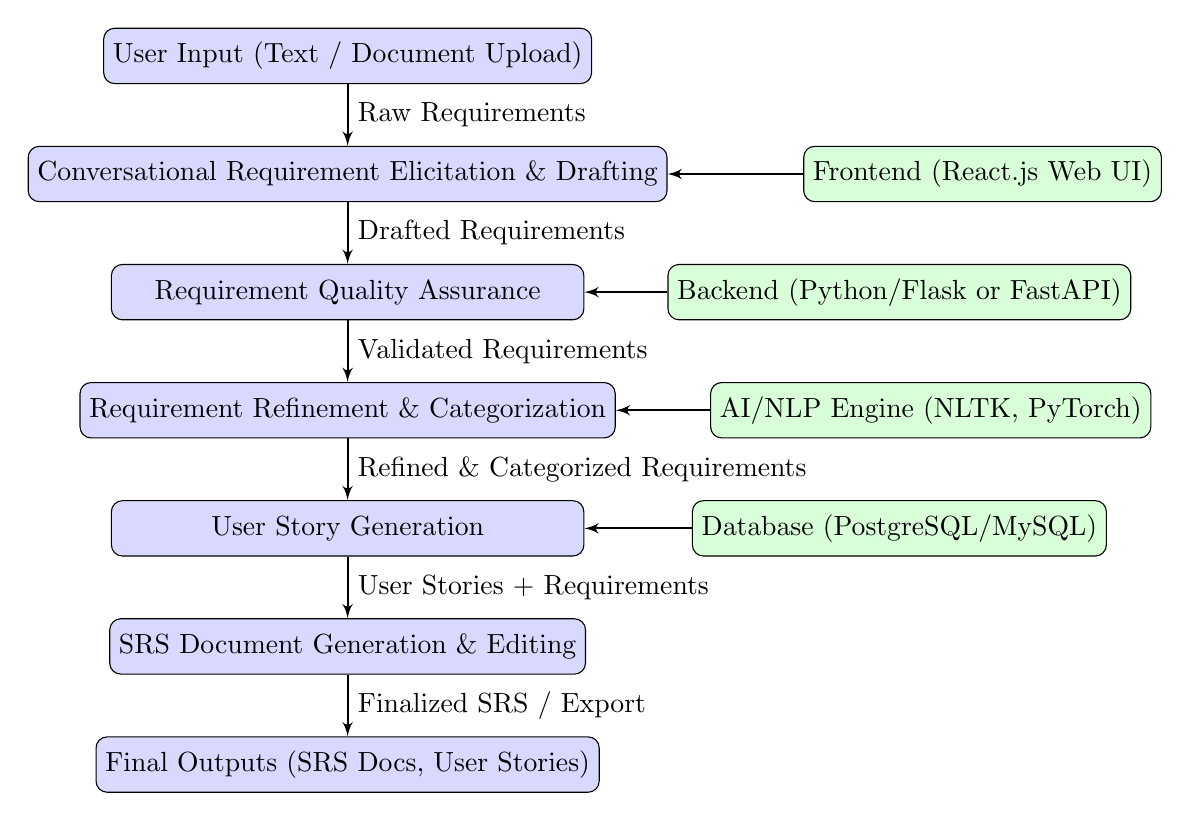
\begin{tikzpicture}[node distance=1.5cm]

% (Minimal fallback styles in case they're not in the preamble)
\tikzstyle{block} = [rectangle, draw, fill=blue!15, text centered, rounded corners, minimum height=2em, minimum width=6cm]
\tikzstyle{line} = [draw, thick, -latex']
\tikzstyle{side} = [rectangle, draw, fill=green!15, text centered, rounded corners, minimum height=2em, minimum width=3cm]

% Main pipeline
\node [block] (input) {User Input (Text / Document Upload)};
\node [block, below of=input] (elicitation) {Conversational Requirement Elicitation \& Drafting};
\node [block, below of=elicitation] (quality) {Requirement Quality Assurance};
\node [block, below of=quality] (refinement) {Requirement Refinement \& Categorization};
\node [block, below of=refinement] (userstories) {User Story Generation};
\node [block, below of=userstories] (srs) {SRS Document Generation \& Editing};
\node [block, below of=srs] (output) {Final Outputs (SRS Docs, User Stories)};

% Arrows (pipes) with labels
\path [line] (input) -- node[midway,right]{Raw Requirements} (elicitation);
\path [line] (elicitation) -- node[midway,right]{Drafted Requirements} (quality);
\path [line] (quality) -- node[midway,right]{Validated Requirements} (refinement);
\path [line] (refinement) -- node[midway,right]{Refined \& Categorized Requirements} (userstories);
\path [line] (userstories) -- node[midway,right]{User Stories + Requirements} (srs);
\path [line] (srs) -- node[midway,right]{Finalized SRS / Export} (output);

% Side components (placed using explicit coordinates relative to pipeline nodes)
\node [side] (frontend) at ($(elicitation.east)+(4cm,0)$) {Frontend (React.js Web UI)};
\node [side] (backend)  at ($(quality.east)+(4cm,0)$)     {Backend (Python/Flask or FastAPI)};
\node [side] (ai)       at ($(refinement.east)+(4cm,0)$)  {AI/NLP Engine (NLTK, PyTorch)};
\node [side] (db)       at ($(userstories.east)+(4cm,0)$) {Database (PostgreSQL/MySQL)};

% Connect side components
\path [line] (frontend.west) -- (elicitation.east);
\path [line] (backend.west)  -- (quality.east);
\path [line] (ai.west)       -- (refinement.east);
\path [line] (db.west)       -- (userstories.east);

\end{tikzpicture}
\caption{Pipe-and-Filter System Architecture of MARS}
\label{fig:architecture}
\end{figure}

The architecture of the proposed system follows a \textbf{pipe-and-filter model}, where each stage of the requirement engineering process is represented as a modular component connected in sequence. User input flows through a series of processing stages, with the output of one stage serving as the input for the next. This ensures that requirements are progressively refined, validated, and transformed into structured artifacts such as user stories and SRS documents.

At the entry point, users interact with the system through a \textbf{frontend web application}, implemented in React.js, which provides both text-based input and document upload options. The frontend connects to the \textbf{backend services}, developed in Python (Flask/FastAPI/Django), responsible for orchestrating workflows and exposing APIs. Core intelligence is handled by the \textbf{AI/NLP engine}, which leverages libraries such as NLTK and PyTorch to perform requirement elicitation, ambiguity detection, conflict resolution, and classification.

Validated requirements and generated artifacts are stored in the \textbf{database layer} (PostgreSQL/MySQL or MongoDB for unstructured storage), ensuring persistence and traceability. The pipeline includes modules for conversational elicitation, quality assurance, refinement, user story generation, and SRS assembly, each functioning as independent but interconnected processing blocks. Additionally, the system integrates a \textbf{document processing component}, using tools like \texttt{python-docx} and Pandoc, to support export into multiple formats such as PDF, DOCX, and Markdown.

This modular architecture promotes scalability, maintainability, and flexibility. For example, improvements to the AI models or integration of new document templates can be performed without affecting the entire system. By adopting the pipe-and-filter design, the architecture ensures that requirements flow in a structured manner from raw input to finalized documentation while maintaining opportunities for human-in-the-loop interaction and feedback.
\section{Tools and Technologies}

\subsection*{Frontend (Web Application Interface)}
\begin{itemize}
    \item React.js  
    \item HTML5, CSS3, JavaScript 
    \item Bootstrap  
\end{itemize}

\subsection*{Backend (Application Logic and APIs)}
\begin{itemize}
    \item Python (Flask/FastAPI/Django)
    \item Node.js (optional)
\end{itemize}

\subsection*{AI/ML and NLP Technologies}
\begin{itemize}
    \item NLTK 
    \item PyTorch 
\end{itemize}

\subsection*{Database and Storage}
\begin{itemize}
    \item PostgreSQL / MySQL 
    \item MongoDB (optional) 
    \item File Storage 
\end{itemize}

\subsection*{Document Processing \& Export}
\begin{itemize}
    \item python-docx 
    \item Pandoc 
\end{itemize}

\section{Work Division}
For each module and respective Feature, assign responsibility to a team member

\begin{table}[!ht]
\caption{Table 1}
\centering
\small
\begin{tabular}{|p{3cm}|p{2cm}|p{9cm}|}
\hline
\textbf{Name} & \textbf{Registration} & \textbf{Responsibility / Module / Featureure} \\ \hline
Mr. Zubair & 22i-2475 & Module 1- Feature 1, Module 2- Feature 1, Module 3- Feature 1, Module 4- Feature 2, Module 5- Feature 3  \\ \hline  
Miss. Arrij & 22i-0755 & Module 1- Feature 2-3, Module 2- Feature 1, Module 3- Feature 2, Module 4- Feature 1, Module 5- Feature 4  \\ \hline  
Miss. Hamna & 22i-1098 & Module 1- Feature 4, Module 2- Feature 3, Module 3- Feature 3, Module 4- Feature 3, Module 5- Feature 2 \\ \hline
Team & - & Module 1- Feature 1, Module 2- Feature 2, Module 5- Feature 1   \\ \hline  
\end{tabular}
\end{table}

\section{Timeline}

\begin{table}[!ht]
\caption{Project Iteration Plan} 
\begin{tabular}{|c|c|p{9cm}|} \hline
\textbf{Iteration \#} & \textbf{Time Frame} & \textbf{Tasks / Modules} \\ \hline
01 & Sept–Oct & Development of Conflict and Duplicate Detection Model, including data preprocessing and validation. \\ \hline
02 & Nov–Dec  & Implementation of Ambiguity Detection, Requirement Classification, and Refinement mechanisms. \\ \hline
03 & Jan–Feb  & Conversational Requirement Elicitation and Automated User Story Generation. \\ \hline
04 & Mar–Apr  & Integration of SRS Editor, Chatbot Interface, Requirement Filtering, and Preliminary Cost–Risk Analysis. \\ \hline
\end{tabular}
\end{table}

%\appendix
% \chapter{Appendix I title}
 
 text here


\bibliographystyle{plain}
\bibliography{bib} 
\addcontentsline{toc}{chapter}{References} 

\end{document}
